\documentclass[14pt,a4paper]{extarticle}
\usepackage[utf8]{inputenc}
\usepackage[T2A]{fontenc}
\usepackage[english,russian]{babel}
%\usepackage{fontspec}
%\setmainfont{Times New Roman} 
\usepackage[unicode]{hyperref}
\usepackage[left=2cm,right=1cm, top=2cm, bottom=2cm]{geometry}
\linespread{1.5}
\usepackage{indentfirst}
\usepackage{amssymb}
\usepackage{cmap}
\usepackage[]{graphicx}
\usepackage{hyperref}
\usepackage{array}
\usepackage{wrapfig}
\usepackage{longtable}
\usepackage{verbatim}
\usepackage{enumitem}
\usepackage{amsmath}
\usepackage{float}
\usepackage{mathtools}
\usepackage{icomma}
\usepackage{caption}
\captionsetup{labelsep=period}
\usepackage{xcolor}
\usepackage{animate}
%\numberwithin{equ`tion}{section}
\newcommand{\ten}[1]{\cdot 10^{#1}}
\hypersetup{
	colorlinks,
	citecolor=black,
	filecolor=black,
	linkcolor=black,
	urlcolor=blue
}

\usepackage{pdfpages}
\newcommand{\whr}{\text{, где}}
\newcommand{\razm}[1]{\hspace{1ex} \ensuremath{\left[\text{#1}\right]}}
\newcommand{\rbf}[1]{\textbf{\ref{#1}}}
\newcommand{\refris}[1]{рис. \rbf{#1}}
\newcommand{\prf}[1]{стр. \textbf{\pageref{#1}}}
\newenvironment{aleq}{\begin{equation}\begin{aligned}}{\end{aligned}\end{equation}}
\renewcommand{\geq}{\geqslant}
\renewcommand{\leq}{\leqslant}
\newcommand{\rt}[1]{_\text{#1}}
\newcommand{\mm}{\razm{мм}}

\renewcommand{\phi}{\varphi}
\renewcommand{\epsilon}{\varepsilon}

\newcommand{\an}[2]{a_{#1}\cos \left({#2}\frac{2\pi x}{P}\right)}
\newcommand{\bn}[2]{b_{#1}\sin \left({#2}\frac{2\pi x}{P}\right)}
\newcommand{\mtrig}[2]{\frac{2}{{#2}\pi}{#1}\left({#2}\frac{2\pi x}{P}\right)}
\author{Максим Зотов}
\title{МТ11-62Б}
\date{Функция передачи модуляции}
\begin{document}
\maketitle
\tableofcontents
\pagebreak
\section{График функции передачи модуляции}
\begin{figure}[H]
	\begin{center}
		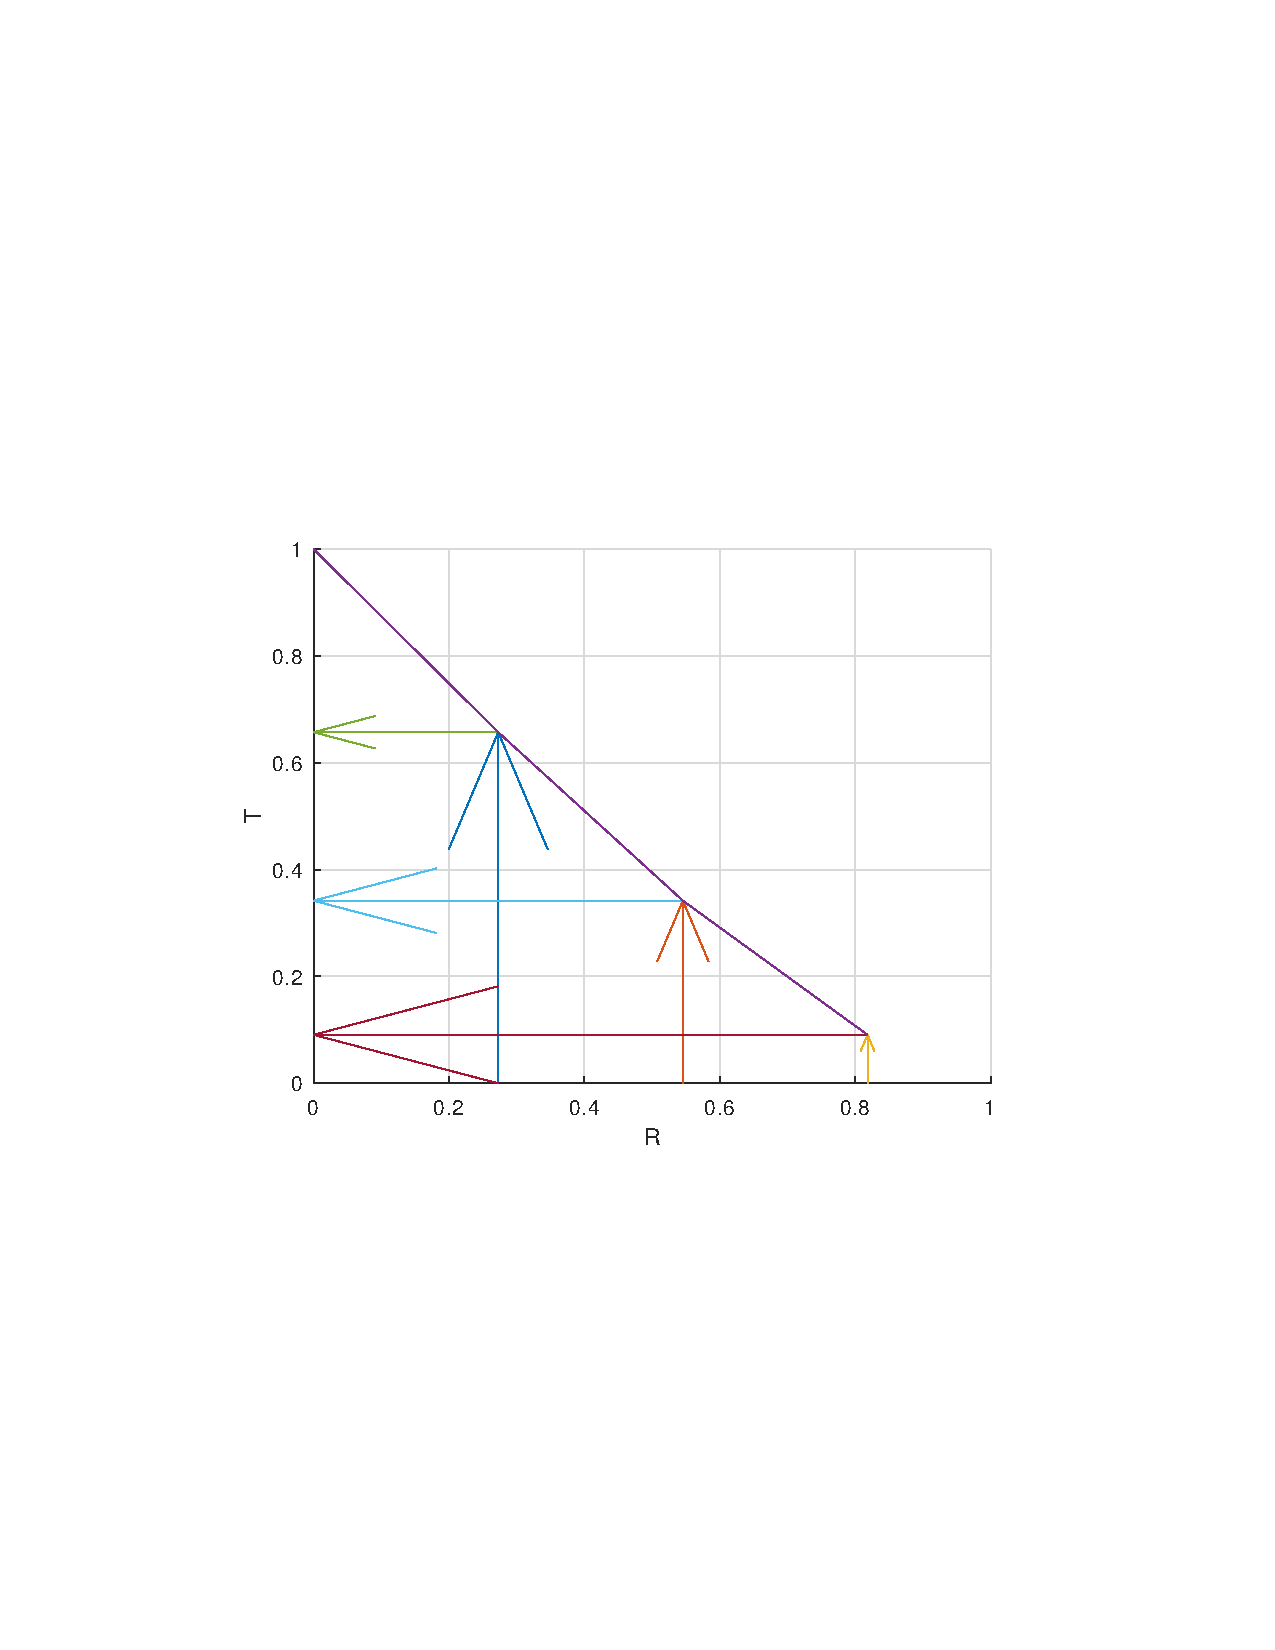
\includegraphics[trim=130 270 130 250,clip, width=\textwidth]{func_mod.pdf}\caption{График ФПМ}\label{fpm}
	\end{center}
\end{figure}
\section{Характеристики выделенных гармоник}
На рисунке ниже показано разложение входного распределения интенсивности на гармоники $(1, 2, 3)$, а также суммарная функция $(1+2+3)$
	\begin{figure}[H]
		\begin{center}
		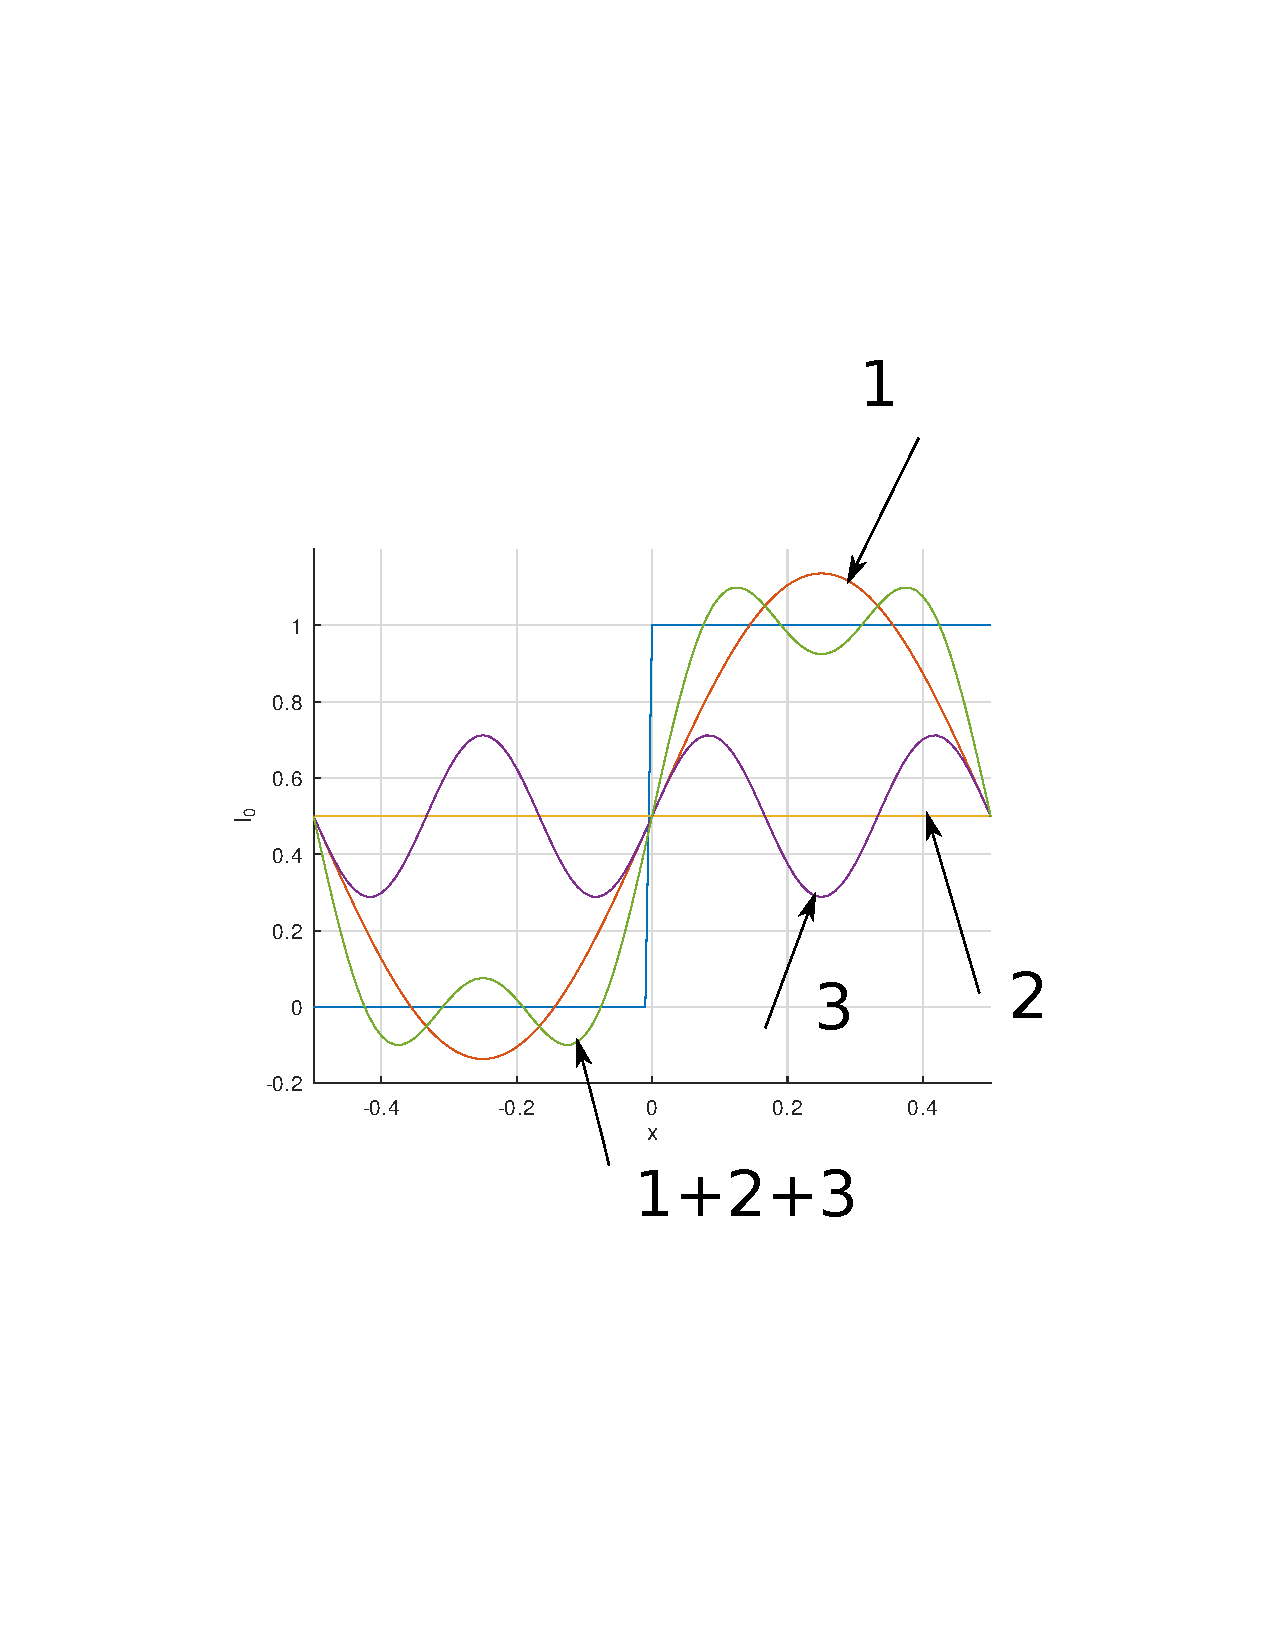
\includegraphics[trim=110 150 110 150,clip, width=0.7\textwidth]{fig1-4e.pdf}\caption{Выделенные гармоники}\label{do}
	\end{center}
	\end{figure}

Частотная характеристика гармоник
\begin{equation}
	\nu=
	\begin{pmatrix}
		1\\
		2\\
		3\\
	\end{pmatrix}
\end{equation}
Значения ОПФ для каждой из гармоник
\begin{equation}
	R = 
	\begin{pmatrix}
		0\\
		0.273\\
		0.545\\
		0.818\\
	\end{pmatrix}\quad\Rightarrow\quad
	T = 
	\begin{pmatrix}
		1\\
		0.657\\
		0.342\\
		0.09\\
	\end{pmatrix}
\end{equation}

\section{Значения амлитуд после прохождения оптической системы}
После прохождения оптической системы амплитуды гармоник несколько уменьшатся. 

Применим обратное Фурье - преобразование для гармоник 1, 2 и 3, получим исходный сигнал, ``исходную'' суммарную функцию $(1+2+3)$
\begin{figure}[H]
	\begin{center}
		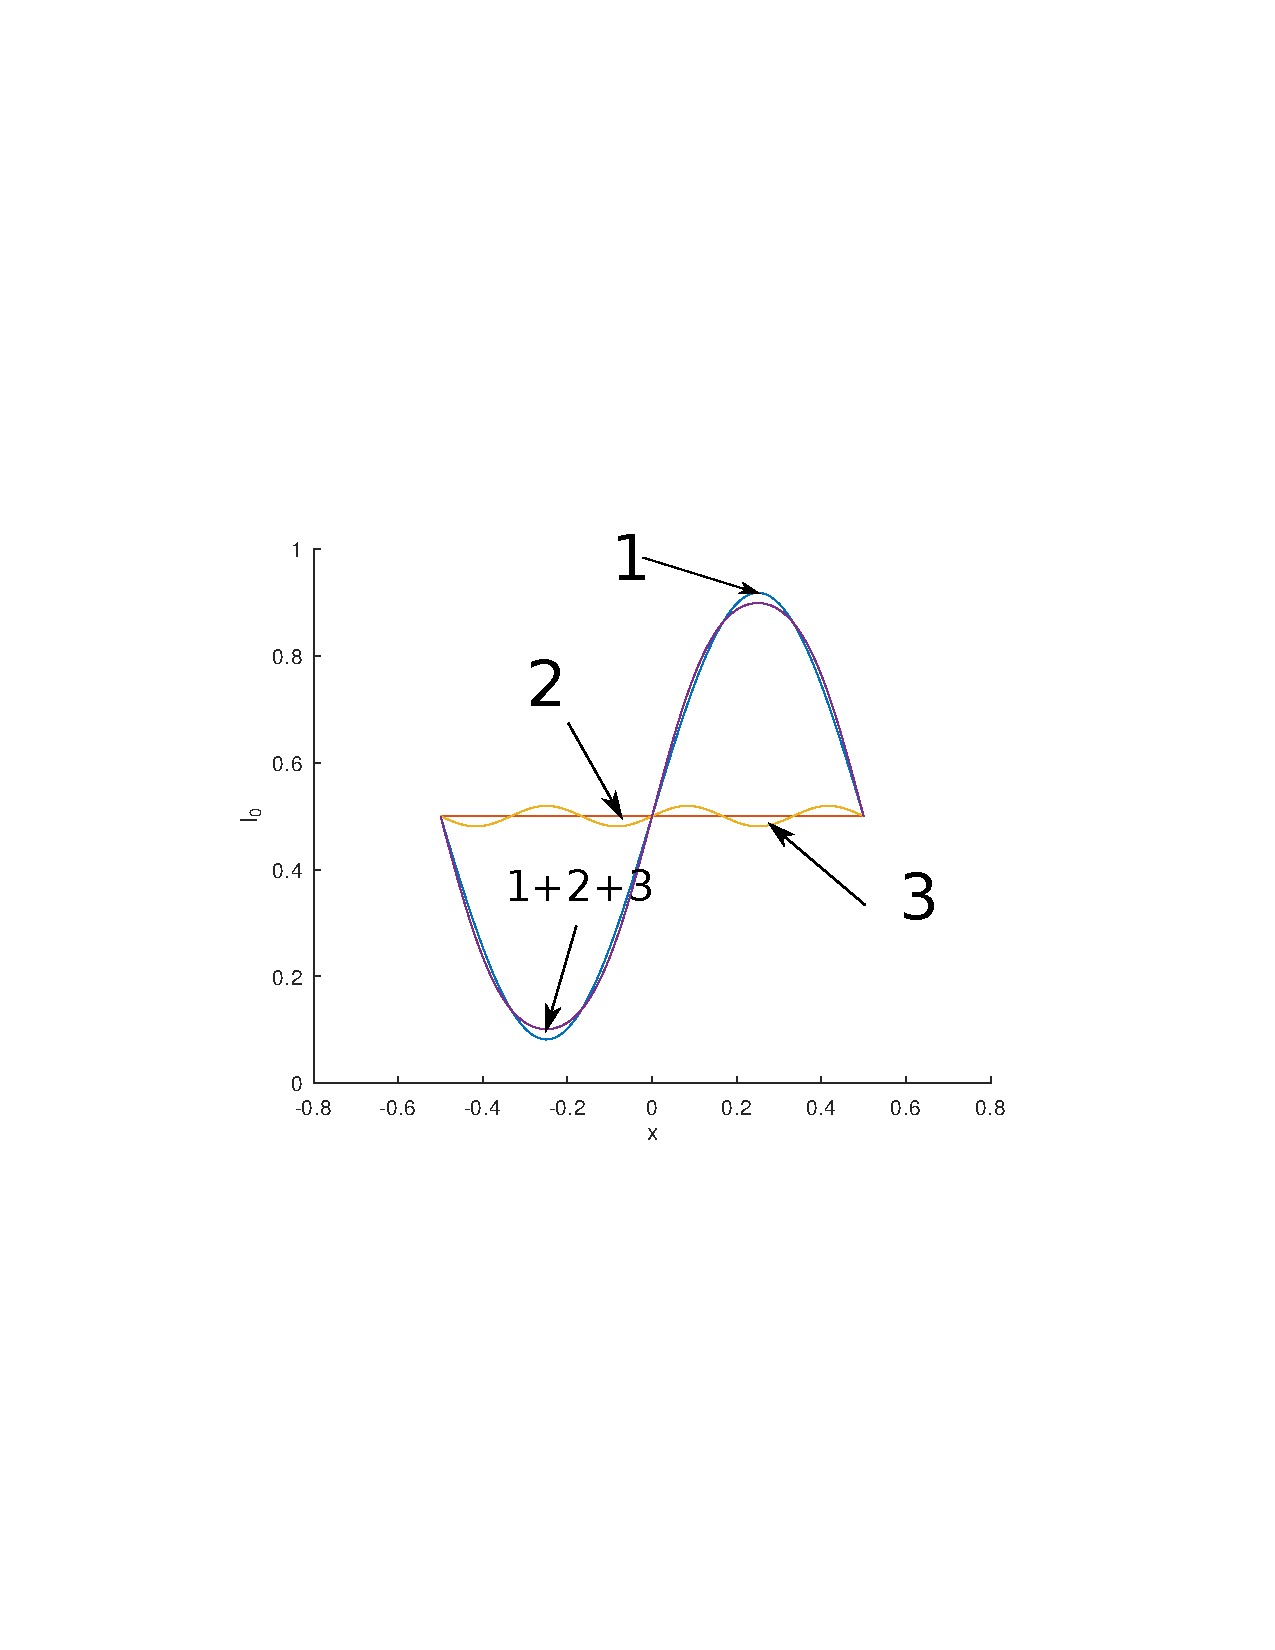
\includegraphics[trim=100 240 100 250,clip, width=0.7\textwidth]{fig4-1e.pdf}\caption{Графики гармоник после прохождения оптической системы}\label{posle}
	\end{center}
\end{figure}
Значения амплитуд после прохождения оптической системы могут быть найдены по тождеству
\begin{equation}
	A_i=\max(T_i f_i)-\min (T_i f_i) \whr
\end{equation}
\begin{itemize}
	\item $T_i$ -- $i$ - я ОПФ
	\item $f_i$ -- $i$ - я гармоника
\end{itemize}

Таким образом
\begin{equation}
	A=\begin{pmatrix}
		0.837\\
		0\\
		0.038\\
	\end{pmatrix}
\end{equation}

Matlab выводит расчёты в следующем формате
\begin{figure}[H]
	\centering
	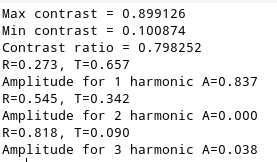
\includegraphics[width=0.7\linewidth]{matlab}
	\caption{Вывод данных из Matlab}
\end{figure}

\section{Графическая иллюстрация обратного Фурье - преобразования}
На \ris{summa} представлены входная функция из \ris{do} (синий цвет), Фурье - разложение до объектива из \ris{do} $(1+2+3)$ и обратное Фурье - преобразование из \rbf{posle} $(1+2+3)$.
\begin{figure}[H]
	\centering
		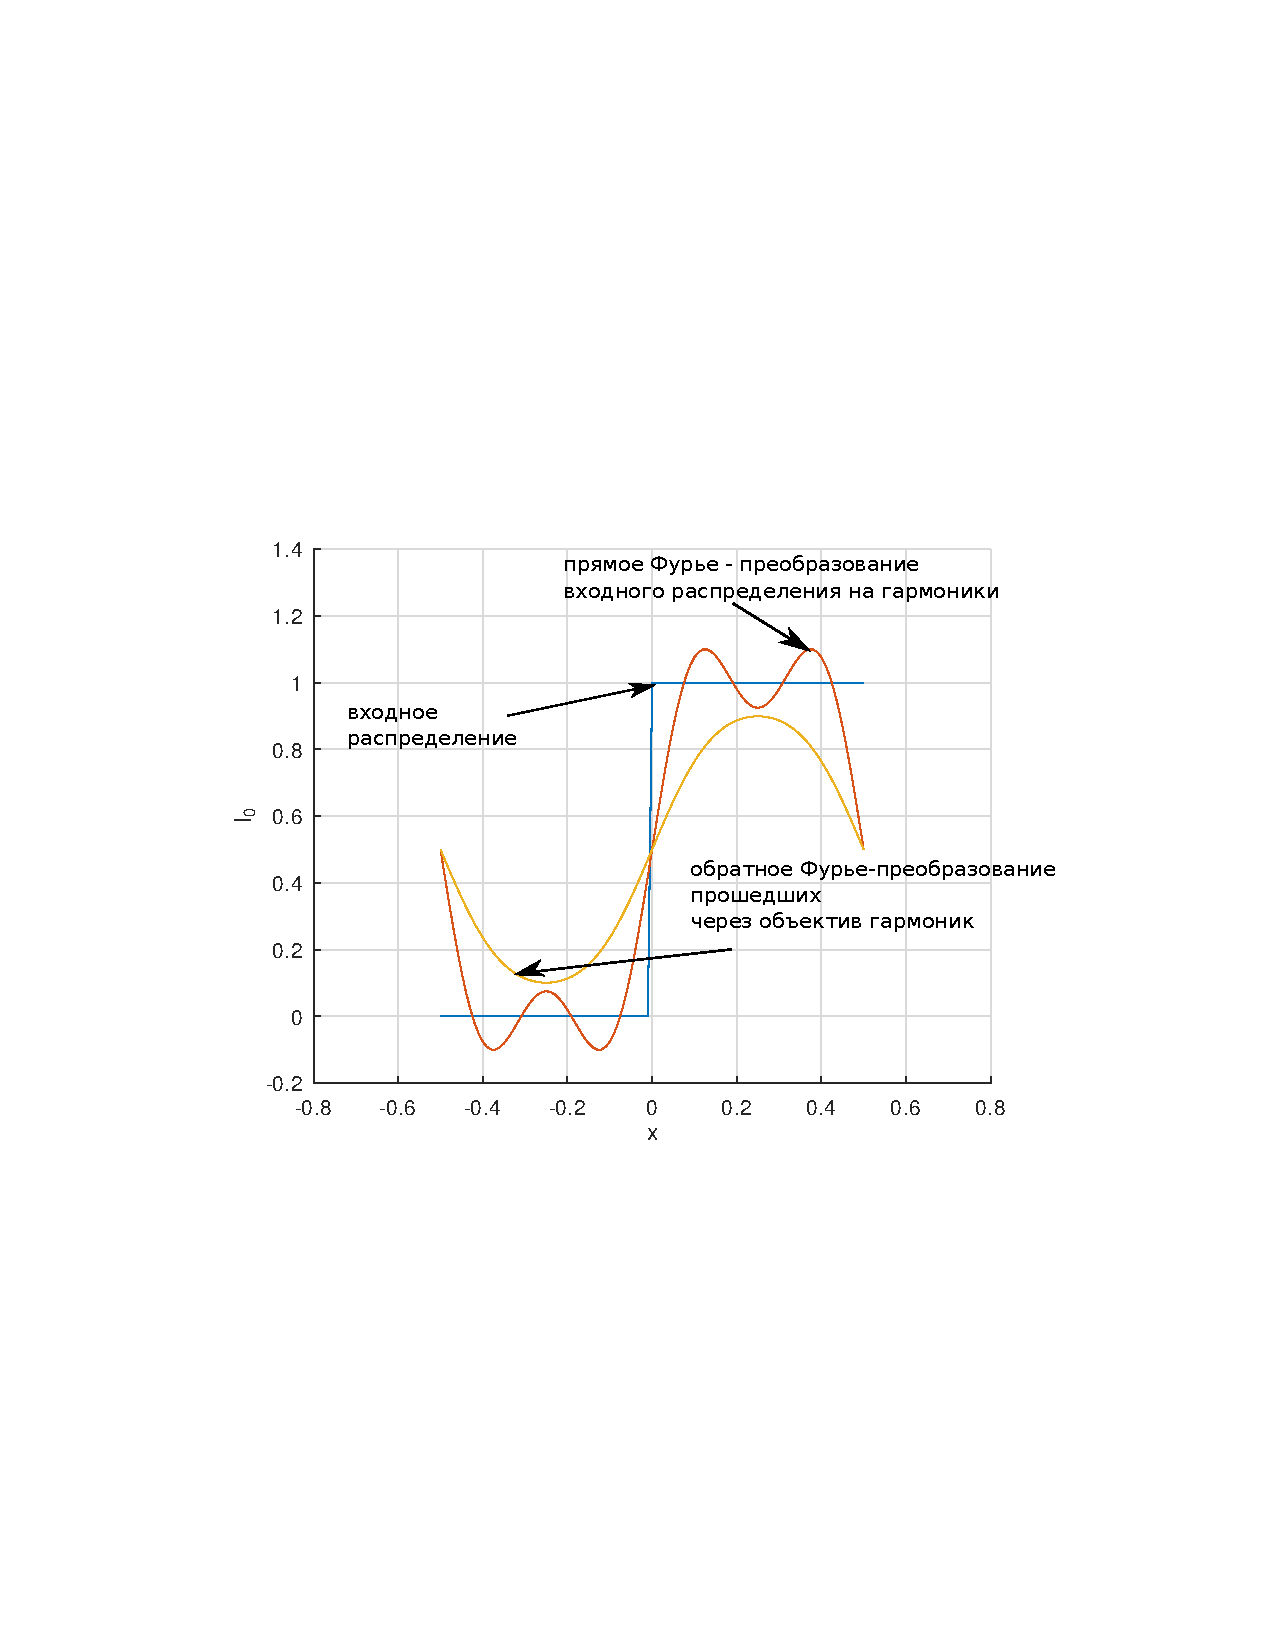
\includegraphics[trim=100 240 100 250,clip, width=0.7\textwidth]{fig5-1e.pdf}\caption{Обратное Фурье-преобразование}\label{summa}
\end{figure}

\section{Выводы}
Обратное Фурье - преобразование позволяет восстановить распределение интенсивности по спектральной характеристике объекта.

В силу того, что объектив пропускал только первые три гармоники, восстановление оказалось не стопроцентным.
\end{document}